\chapter{Introduction}
\label{indledning}

The containers freighted by the maritime sector in 2013, amounts to more than 651 million twenty foot equivalent units (TEU). All of these containers are being loaded to and from ships by ship to shore (STS) cranes. The time it takes to transit, containers are thus dependent on the speed of which the cranes can move a container, from one position to another, henceforth called the efficiency of the crane. Increasing the efficiency of the crane leads to greater profitability, as ships need to stay passively in the harbor for a smaller period of time. To increase the efficiency of the crane, higher acceleration is needed when moving the container, which leads to an issue. The issue being that the acceleration of the containers results in the container swinging, the reason for this swinging is that the container acts as a pendulum. When the cart on top of the pendulum is moved, the angle of the pendulum is changed, which causes the pendulum to swing. This is illustrated on \figref{IntroductionPic}.
\begin{figure}[H]
\centering
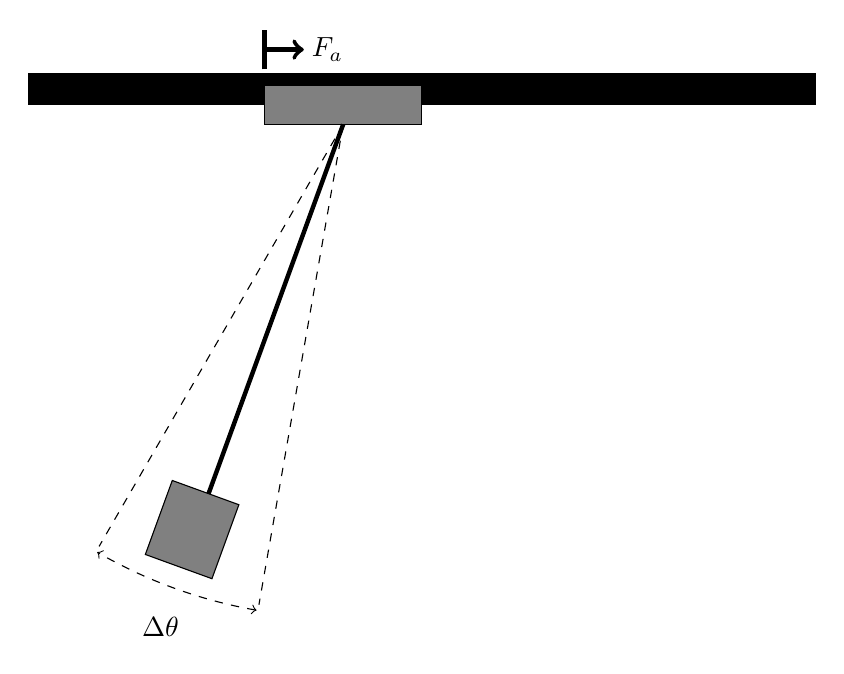
\begin{tikzpicture}
	\draw [ultra thick] (-1,0.7) -- (-1,1.2);
	\draw [->,ultra thick] (-1,0.95) -- (-0.5,0.95);
	\node at (-0.2,0.95) {$F_a$};
	\node at (-2.32,-6.38) {$\Delta \theta$};
	

	\draw [fill = black] (-4,0.25) rectangle (6,0.65);
	\draw [fill = gray] (-1,0) rectangle (1,0.5);

	\draw [dashed] (0,-0) -- (-1.07,-6.1); % 260
	\draw [ultra thick] (0,0) -- (-1.71,-4.69);  % 250
	\draw [dashed] (0,0) -- (-3.1,-5.36);   % 240

	\draw [<->,dashed] (-1.1,-6.17) arc [radius=6.2, start angle=260, end angle= 240];

	\draw[fill = gray,rotate around={-20:(-1.71,-4.69)}] (-2.2,-4.69) rectangle (-1.3,-5.69);
\end{tikzpicture}
\caption{Illustration of the cargo oscillating between two angles when a force is applied to the cart.}
\label{IntroductionPic}
\end{figure}


% \begin{figure}[H]
% \centering
% \includegraphics[width=0.5\textwidth]{missingfigure}
% \caption{}
% \label{fig:intro_fig}
% \end{figure}


%\cite{quad_bevaegelse}

Firstly, a swinging container stresses the equipment. Secondly, a swinging container is hard to place properly. Increasing the efficiency of the cranes can thus be approached in two ways. One being solely increasing the stability of the container hanging from the crane, thus minimizing the swinging caused by faster placement of the container. This would be an assistant system for the operator. The other method is an automatic system, that not only stabilizes the container, but also optimizes the route of the container, as well as the acceleration and deceleration to get the fastest possible relocation of the containers, further increasing the efficiency of the crane.
Of the two possibilities this project will from here on focus on creating an automatic control system which can operate a crane. This project is based on a model crane which is provided by Aalborg University. This leads to the following problem statement:

\begin{itemize}
\item How can a control system be designed to automatic operate a crane.
\end{itemize}

In the following, analysis on how the crane is working and how it reacts when a force is applied is studied. A design for a controller is derived, simulated and tested to see if it is possible to design an automatic controller with the tools of classic controller theory. 
